\documentclass{article}

% Language setting
% Replace `english' with e.g. `spanish' to change the document language
\usepackage[english]{babel}

% Set page size and margins
% Replace `letterpaper' with `a4paper' for UK/EU standard size
\usepackage[a4paper,top=2cm,bottom=2cm,left=3cm,right=3cm,marginparwidth=1.75cm]{geometry}

% Useful packages
\usepackage{amsmath}
\usepackage{graphicx}
\usepackage[colorlinks=true, allcolors=blue]{hyperref}

\title{Project 2 - Synchronization}
\date{CECS 326 - Operating Systems}

\begin{document}
\maketitle

\begin{center}
	\begin{tabular}{l r}
		Due Date: & March 16, 2023 \\ % Date the lab due
		Contributors: & Twan \textsc{Tran} \\ % Partner names
		&  Bharath \textsc{Varma Kakarlapudi} \\
		Instructor: & Hailu \textsc{Xu} % Instructor/supervisor
	\end{tabular}
\end{center}

\section{Lab Summary}

This lab involves implementing a solution to the dining-philosophers problem using monitors, either with POSIX mutex locks and condition variables or Java condition variables. The problem involves five philosophers, each identified by a number 0\dots 4, and each philosopher runs as a separate thread. The philosophers alternate between thinking and eating, and to simulate both activities, each thread sleeps for a random period between one and three seconds.

\subsection{Objective}
The goal of this lab is to provide a solution to the dining-philosophers problem and to demonstrate how to implement it using monitors.

\subsection{Design}
In this lab, we implemented a solution to the Dining Philosophers problem using Java. We used the ReentrantLock, Lock and Condition classes to implement a shared monitor between the philosophers. The DiningServerImpl class is responsible for handling the synchronization between the philosophers, while the Philosopher class represents each philosopher thread. And lastly, the Philosopher class represents each philosopher thread, which alternating between eat, sleep, think.

\section{Implementation}

\subsection{DiningServer.java (Bharath)}

The DiningServer interface provides an interface that will be implement in DiningServerImpl class. It contains the methods for the philosophers to communicate with the DiningServer object. In the dining-philosophers problem, the DiningServer is responsible for coordinating access to the shared resources, which in this case are the forks on the table. The takeForks() method is called by a philosopher when they want to eat, and returnForks() is called when they are finished eating and ready to return the forks back on the table.

\subsection{DiningServerImpl.java (Twan)}

The DiningServerImpl class implements the DiningServer interface, which contains the methods called by the philosophers. It uses the ReentrantLock, Condition, and Lock classes from the java.util.concurrent.locks package. The constructor initializes the lock, forks, and available boolean arrays, and creates a Condition object for each fork using lock.newCondition().

The takeForks() method is called by a philosopher when they wish to eat. It first locks the monitor using the lock.lock() method, then calculates the index of the left and right forks based on the philosopher number. It enters a while loop that waits for both forks to be available using the await() method on each fork's Condition object. When both forks are available, it sets the forks to unavailable, prints a message indicating which forks are with which philosopher, and unlocks the monitor using the lock.unlock() method.

The returnForks() method is called by a philosopher when they are finished eating. It first locks the monitor using lock.lock(), then sets both forks to available, signals the Condition objects for each fork using the signal() method, and unlocks the monitor using lock.unlock().

This implementation ensures that only one philosopher can hold a fork at a time, and that no two adjacent philosophers hold their respective left forks at the same time, thus preventing deadlock.
\subsection{DiningPhilosophers.java (Bharath)}

The DiningPhilosophers class has the main class of the program that starts the dining philosophers problem. It creates 5 philosopher threads and a DiningServerImpl object which implements the DiningServer interface.

In the main() method, it first creates a DiningServerImpl object with the number of philosophers as the argument. Then, it creates an array of Philosopher objects and assigns each object a unique philosopher number and the DiningServerImpl object. Finally, it starts each philosopher thread by creating a new thread object and passing the corresponding Philosopher object as the target.

\subsection{Philosophers.java (Twan)}

The Philosopher class represents each philosopher thread. The run() method is called when the thread starts, and it loops indefinitely, alternating between taking forks, eating, returning forks, and thinking. The eat() and think() methods sleep for a random amount of time from 1-3s to simulate the philosopher eating and thinking.

\section{Result}
\subsection{Output}

\begin{figure}[!h]
\centering
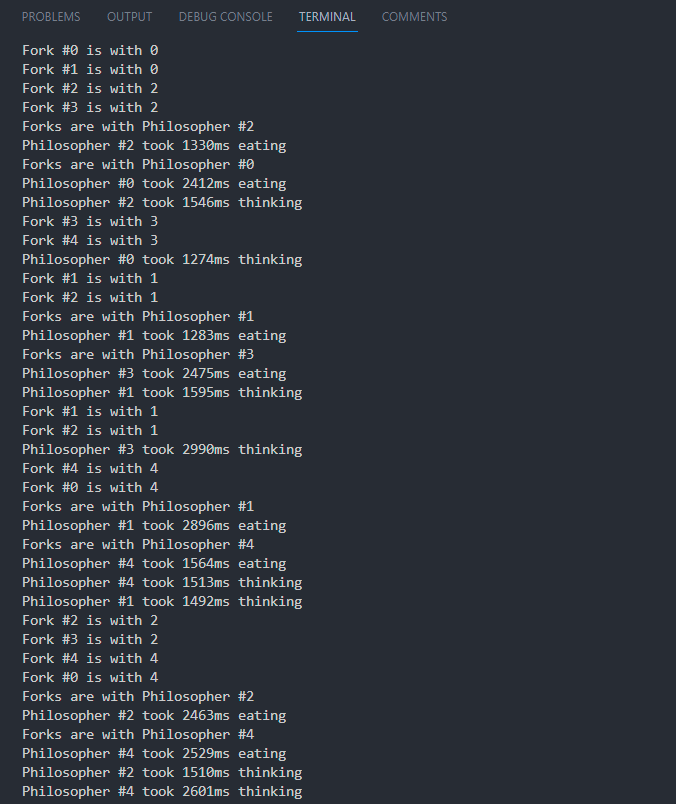
\includegraphics[scale = 0.4]{fig1.png}
\caption{\label{fig:output}This is the output of the program after it ran.}
\end{figure}

The output is showing the actions of each philosopher in the Dining Philosophers problem. Each philosopher alternates between eating and thinking, and must acquire two forks to eat, which represent the resources being shared.

The output also shows the different times each philosopher spends eating and thinking, as well as which forks are being used at any given time. The random sleep times are meant to simulate a more realistic scenario where each philosopher doesn't always behave exactly the same way.

\subsection{Demonstration (Twan)}

Link: \href{https://www.youtube.com/}{YouTube}

\end{document}